\chapter{Results and their Discussion}
In this chapter we present the results of the experiment performed in order to evaluate the incidence of each class of ambiguity in NFA'a obtained from converting regular expressions. We considered two standard methods: Glushkov (also known as Position) \cite{glu61} and Antimirov (also known as Partial Derivatives or PD) \cite{Antimirov96}.
 % order to find the relation between the classes of ambiguity and the size of the automaton.

To perform the experiment $10000$ regular expressions were generated for each $n \in \{20$, $35$, $50$, $75$, $100\}$ and $k \in \{2$, $5$, $10\}$, where $n$ is the number of symbols in the expression excluding parentheses and $k$ is the size of the alphabet. Each regular expression was converted into two NFA's, one for each method of conversion.

% After the regular expressions were generated, for each one of them, we converted it to an NFA with the methods of \emph{Position} and \emph{Partial Derivatives} getting two NFA's .

The average size of the automata resulting from the conversion using the \emph{Position} method is $n/2$ and using the \emph{PD} method is $n/4$, where $n$ is the size of the regular expression \cite{BrodaMMR11}.

We classified the NFA's using the algorithms explained in the last chapter. The results are summarized in Figure \ref{fig:results}.

In the graphics of Figure \ref{fig:results} we can see that both methods have similar distributions. That was expected because it was proven that the \emph{PD} automaton is isomorphic to a quotient of \emph{Position} automaton \cite{IlieY03}.

The number of \emph{unambiguous automata} increases if the $k$ is large or when the $n$ is small.

In our results, PNFA is the class of ambiguity with the lowest presence.

Contrary to the \emph{unambiguous} automata, the number of \emph{exponential ambiguous} automata increases if the $n$ is large or when the $k$ is small.

\begin{figure}[]
  \hspace*{-2.3cm}
  \centering
  \begin{tabular}{cc}
    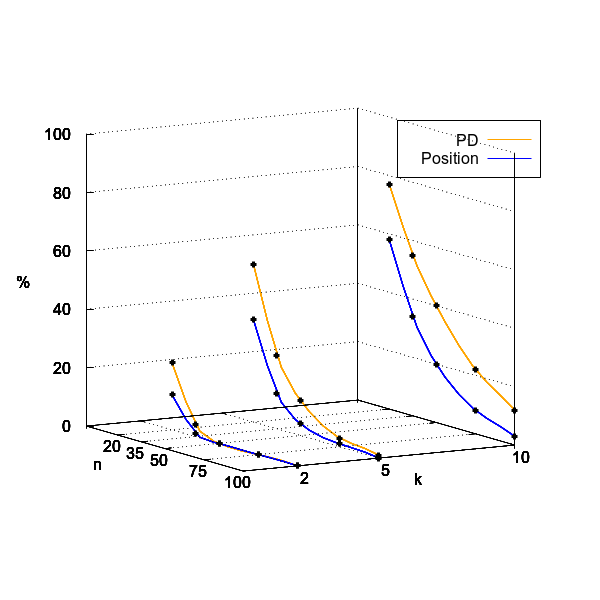
\includegraphics[width=0.6\columnwidth]{ufa} &   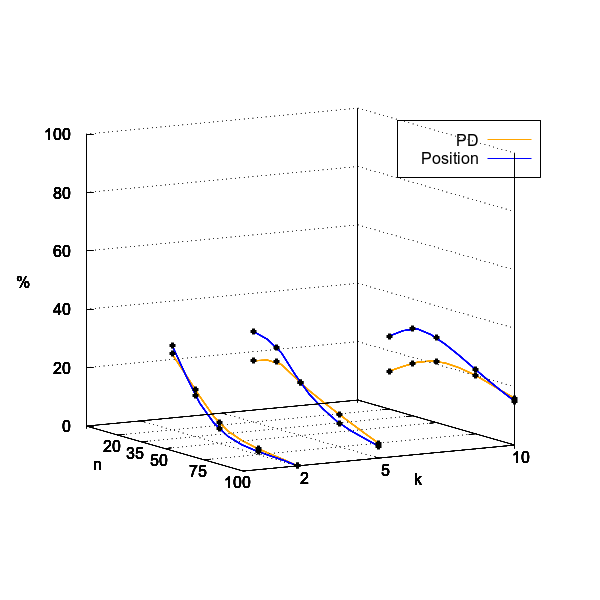
\includegraphics[width=0.6\columnwidth]{fnfa} \\
  (a) Unambiguous Automata & (b) Finitely Ambiguous Automata \\[6pt]
   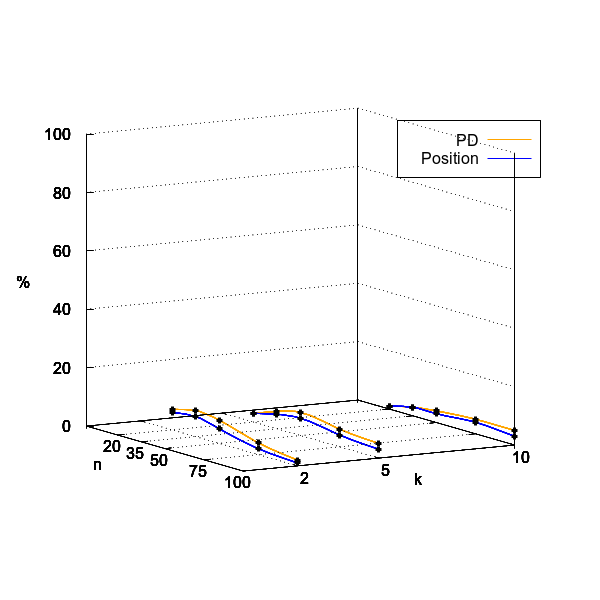
\includegraphics[width=0.6\columnwidth]{pnfa} &   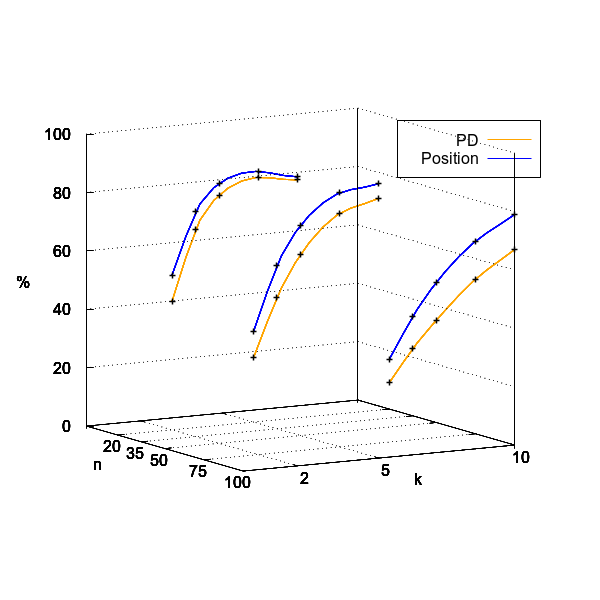
\includegraphics[width=0.6\columnwidth]{enfa} \\
  (c) Polinomially Ambiguous Automata & (d) Exponentially Ambiguous Automata \\[6pt]
  \end{tabular}
  \caption{Results}
  \label{fig:results}
\end{figure}
